\documentclass[12pt]{book} 

\usepackage{amsmath}
\usepackage{graphicx}
\usepackage{import}
\usepackage{amsfonts}
\usepackage{booktabs}

\setlength{\parindent}{0em}  % sets auto indent at new paragraph to none

\newcommand{\incfig}[1]{%
        \import{./figures/}{#1.pdf_tex}
}

\newcommand{\incimg}[2]{%
       \begin{figure}[h]
               \centering
               \includegraphics[scale = #2]{./figures/#1}
       \end{figure}
}

\title{\coursetitle\linebreak\lecturename}
\author{\\Cain Susko\\ 
           \\ \\ \\
      Queen's University 
    \\School of Computing\\} 

%=-=-=-=-=-title-=-=-=-=-=%
\newcommand{\lecturename}{Unsupervised Learning: K-Means Clustering}
\newcommand{\coursetitle}{Linear Data Analysis}
%=-=-=-=-=-#####-=-=-=-=-=%

\begin{document}
\begin{titlepage}
        \maketitle
\end{titlepage}


\section*{a A Conceptual Hierarchy of Machine Learning}
the main concepts of thislecutre are:
Hpyer planes, learning through clustering, the k-means algorithm.

we will use a simple Hierarchy of machine learning. there are 2 heirarchies:
\begin{itemize}
        \item Unsupervised - find natural clusters
                \begin{itemize}
                        \item Binary Clustering
                        \item Multi-Class CLustering
                \end{itemize}
        \item Supervised - cluster using predetermined labels
                \begin{itemize}
                        \item Binary Labelling
                        \item Multi-Class Labelling
                \end{itemize}
\end{itemize}

\section*{b Hyperplane of Seperation}
in 2D, we can seperate data with a line, in 3D we can seperate data with a plane. in $N$ dimensions we can seperate data using a 
hyperplane.

A hyper plane is a vector space + a reference point

\begin{align*}
        &2D &line\;\;\;\;\;\;&\vec l(z) = \vec r + z\vec d\\
        &3D &plane\;\;\;\;\;\;&\vec p(z) = \vec r + z_1\vec d_1 + z_2\vec d_2 
\end{align*}

Suppose $\mathbb{R}^m$. The Hyperplane $\mathbb{H}$ is defined as point $\vec v$ is in $\mathbb{H}$:

for $\vec w\neq \sigma$ and $b\in \mathbb{R}$:

\[\vec w \cdot \vec v + b = 0\]
\[\vec w \cdot \vec v = -b\]

where $\vec w$ is the \textbf{normal vector} and $b$ is the \textbf{biased scalar}.
We may also sometimes need the unit normal vector, which is:
\[\vec n \cdot \vec v = -a\]

\subsection*{HyperPlane Partitioning}
given the point $\vec u \in \mathbb{R}^m$ and the hyperplane $\mathbb{H}: \vec h, \vec r$

to find out if $\vec u$ is on one side or the other of $\mathbb{H}$, we must project the reference point $\vec r$ and the point $\vec u$ into the 
vectorspace of the hyperplane: $\vec h$.
\begin{align*}
        (\vec u - \vec r) \cdot \vec h &= \vec h \cdot (\vec u - \vec r)\\
                                       &=\vec h \cdot \vec u - \vec h \cdot \vec r\\
                                       &=\vec h \cdot \vec u + a
\end{align*}

and thus, we will define $\vec u$ to be on the positive side of $\mathbb{H}$ because $\vec h \cdot \vec u + a \geq 0$
so do we need a unit normal? (see the final equation in $b$). Recall a inequality holds if both sides are multiplied by the same factor.

thus, if $\vec u$ is in the positive side of $\mathbb{H}$ then:
\[\vec h \cdot \vec u + a \geq 0\]

additionally, let $\vec w = ||\vec w||\vec h$. therefore:
\begin{align*}
        ||\vec w||(\vec h \cdot \vec u + a) &\geq ||\vec w||0\\
        \equiv ||\vec w||(\vec h \cdot \vec u) + b &\geq 0\\
        \equiv \vec w \cdot \vec u + b &\geq 0
\end{align*}
so what does this tell us? from evaluating the equation 
$\vec w \cdot \vec u + b$, if the result is positive, the point 
$\vec u$ is in the positive side of $\mathbb{H}$ and if the 
result is negative, $\vec u$ is on the negative side.

Also note that, $\vec h \cdot (\vec u - \vec r)$ is the orthogonal 
distance from $\vec u$ to the hyperplane $\mathbb{H}$

\paragraph{Example}
suppose were given a unit normal: 
$\vec h = \begin{bmatrix} 1\\0 \end{bmatrix}$ with a reference point of 
$\vec r = \begin{bmatrix} 2\\0 \end{bmatrix}$ 
and a biased scalar of $a = -2$.
we know that $\vec h \cdot \vec u$ equals the first entry of $\vec u$:
\[\vec h \cdot \vec u = u_1\]
this thus implies that:
\[\vec h \cdot \vec u + a \geq 0 \equiv u_1-2 \geq 0 \equiv u_1 \geq 2\]
thus we can say that any point who's first entry is greater than 2 is on 
the positive side of $\mathbb{H}$ and everything with first entry less
than 2 is on the negative side of $\mathbb{H}$

\paragraph{Example}
given:
\[\vec w = \begin{bmatrix}1\\1\end{bmatrix}, b = 2\]
now, say the point is the zero vector, then:
\[\vec w \cdot \begin{bmatrix} 0\\0\end{bmatrix} + 2 \geq 0\]
thus, the origin (0,0) is on the positive side of this hyperplane.
\incimg{decision}{0.5}
we can view $\mathbb{H}$ as a line or a `decision' that the model will
make.
\pagebreak

\section*{c Basics of Vector Clustering}
we shall expolre Vector Clustering. Assume a data vector is: $\vec x \in 
\mathbb{R}^m$

Additionally, a cluster is:
\begin{itemize}
        \item A set $s_i$ with $\vec x_j$ entries or
        \item A centriod $\vec g_i$ with neightbors.
\end{itemize}
Note: we will primarily use the \textbf{centriod} definition 
of a cluster
\paragraph{What is a Cluster}
thus, the question is; how do we define a cluster?
A simple approach we can use is to treat vectors uniformly or\\
we can treat vectors hierarchically, meaning we will allow 
subsets.

\paragraph{$l_2$ Centriod of a Set}
the concept is to associate the centriod (e.g. mean) with a cluster
$S_i$ which is written as $\vec g_i$. We can do this in 2 ways:
\begin{itemize}
        \item[i] Define mean in terms of cluster
\[\vec g_i =^{def} \frac{\sum_{\vec u\in S_i}\vec u}{m_i}\]
        \item[ii] Define cluster in terms of mean
\[S_i =^{def} \{\vec u \mid \forall_l ||\vec u - \vec g_i||^2 
\geq ||\vec u - \vec g_l||^2\}\]

note that $m$ is the mean of the vector. and $||x - y||^2$ is the 
distance between the points $x, y$
\pagebreak


Observe the below example of clustering:
\begin{figure}[h]
        \centering
        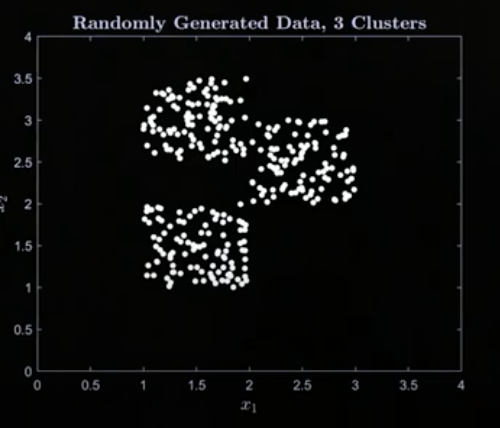
\includegraphics[scale=0.5]{./figures/cluster1.png}
        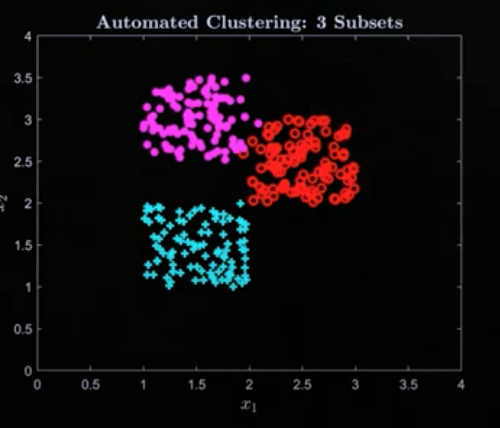
\includegraphics[scale=0.5]{./figures/cluster2.png}
\end{figure}

The number of clusters matters, as without the magenta, part of the 
magenta cluster would be clustered in with the red instead.

Funrthermore, clustering can change depending on new data, as the
clusters' bounds will change with new points.
\end{itemize}

\section*{d K-Means Clustering}
in clustering a problem that often comes up is: how many sets do we use?
Usually, the user gives us this number as $k$ such that:
\[S = S_1, S_2, ..., S_k\]

the difficulty is for $\vec x \in \mathbb{R}^m$ the complexity is $O(m^{nk+1})$


Instead, we will use Lloyd's k-means algorithm, which has a complexity of
\[O(mnkl)\]

where $m$ is for the number of entries in each vector. $n$ for each vector.
$k$ for each cluster, and $l$ for each iteration.

the code for this in MatLab would be:
\begin{verbatim}
        kmeans(Xmat, k)
\end{verbatim}

\paragraph{Recall}
that a cluster is either a set $S_i$ with $\vec x_i$ entries or 
a centriod $\vec g_i$ with neighbors.

\paragraph{Consider}
altering these defintions. For example: initialize contriods $\vec g_i$.
The pseudo-code for this would be:
{\small
\begin{verbatim}
while not converged:
        for each vecx_j:
                assign index i of nearest vecg_i
                for each i:
                        compute vecg_i from points w/ index i
\end{verbatim}
}
Note: the vector norm matters (ie. $L_2$ norm vs. Frobenius norm).
for the Euclidian norm $L_2$ use the mean of $\vec x_i$. for the 
Manhattan norm $L_1$ use the median of $\vec x_i$

\section*{Clustering the Iris Data}
this section will explore the best known dataset in machine learning: Fisher's
Iris Data Set.

in MatLab, we can use \texttt{load fisheriris}. to get the data from there,
we will use \texttt{Xmat = meas(:, 3:4);} to extract columns 3 and 4 from
the data set. 

What we want to do is find the index array and the row oriented centiods (means)
for $k=2$: \texttt{[kidx, kmrow] = kmeans(Xmat, 2)}

finally, we can plot the results

\begin{figure}[h]
        \centering
        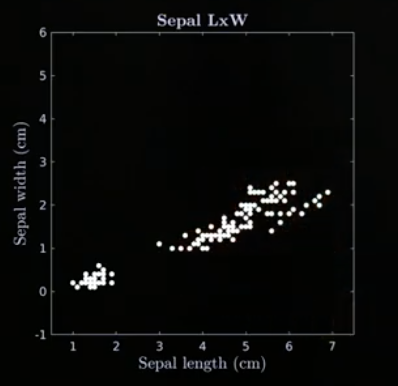
\includegraphics[scale=0.5]{./figures/iris1.png}
        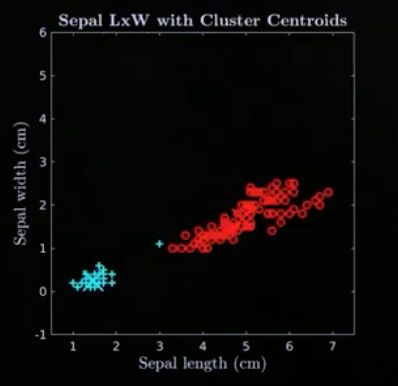
\includegraphics[scale=0.5]{./figures/iris2.png}
        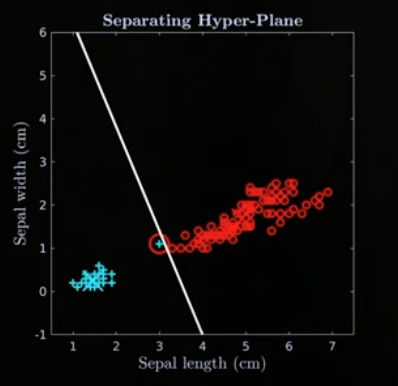
\includegraphics[scale=0.5]{./figures/iris3.png}
\end{figure}

But We can see that there is a cyan data vector that is beyond the bounds of
the majority of the cyan cluster.
\pagebreak

But this can be explained by a seperating hyper-plane that partitions that 2
clusters. For every 2 centriods, there is a hyper-plane that divides them.
\end{document}

